% !TEX encoding = UTF-8
\documentclass[a4paper,12pt]{extarticle}
\usepackage[utf8]{inputenc}
\usepackage[T2A]{fontenc}
\usepackage[russian]{babel}
\usepackage{geometry}
\geometry{left=25mm, right=10mm, top=20mm, bottom=20mm}
\usepackage{setspace}
\onehalfspacing
\usepackage{indentfirst}
\usepackage{tempora} % Аналог Times New Roman
\setlength{\parindent}{1.25cm}
\usepackage{amsmath,amssymb}
\usepackage{graphicx}
\usepackage{listings}
\usepackage{xcolor}
\usepackage{hyperref}
\usepackage{longtable}
\usepackage{booktabs}
\usepackage{array}
\usepackage{caption}
\captionsetup[table]{labelsep=endash, justification=raggedright, singlelinecheck=false}
\renewcommand{\tablename}{Таблица}
\usepackage{enumitem}
\usepackage{float}

\lstset{
  basicstyle=\ttfamily\small,
  breaklines=true,
  frame=single,
  backgroundcolor=\color{gray!10},
  keywordstyle=\color{blue},
  commentstyle=\color{green!50!black},
  stringstyle=\color{red!70!black},
  showstringspaces=false,
  language=Python
}

\usepackage{microtype} % Улучшенные переносы и spacing
\usepackage{ragged2e} % Для корректного выравнивания

% Разрешить LaTeX более гибко переносить строки
\tolerance=1000
\emergencystretch=3em
\hfuzz=1pt

% Переносы URL на любых символах
\makeatletter
\g@addto@macro{\UrlBreaks}{\UrlOrds}
\makeatother

\hypersetup{colorlinks=true,linkcolor=black,urlcolor=blue,citecolor=black,breaklinks=true}

\begin{document}

% ==================== TITLE PAGE ====================
\begin{titlepage}
\thispagestyle{empty}
\begin{center}
ПРАВИТЕЛЬСТВО РОССИЙСКОЙ ФЕДЕРАЦИИ \\
ФГАОУ ВО НАЦИОНАЛЬНЫЙ ИССЛЕДОВАТЕЛЬСКИЙ УНИВЕРСИТЕТ \\
\textbf{\guillemotleft ВЫСШАЯ ШКОЛА ЭКОНОМИКИ\guillemotright} \\[0.5cm]
Факультет компьютерных наук \\
Образовательная программа \guillemotleft Прикладная математика и информатика\guillemotright \\[2.5cm]
\textbf{\Large Отчет об исследовательском проекте на тему:} \\[0.5cm]
\textbf{\large Применение обучения с подкреплением\\в исследовании игр в автобаттлерах} \\[3cm]
\end{center}
\vfill
\begin{flushright}
Выполнил: \\
студент группы БПМИ243 \\
Пономарев Тимур Евгеньевич \\[1cm]
Приняли руководители проекта: \\[0.3cm]
к.ф.-м.н. \\
Кудеров Пётр Викторович \\[0.7cm]
Старший преподаватель \\
Департамента больших данных \\
и информационного поиска \\
Горденко Мария Константиновна \\
\end{flushright}
\vfill
\begin{center}\textbf{Москва 2026}\end{center}
\end{titlepage}

\newpage
\tableofcontents
\newpage

% ==================== ANNOTATION ====================
\section*{Аннотация}
\addcontentsline{toc}{section}{Аннотация}

Автобаттлеры --- класс стратегических игр с неполной информацией, стохастическими переходами состояний и комбинаторно обширным пространством действий, представляющий одну из открытых задач в области обучения с подкреплением (Reinforcement Learning, RL). Hearthstone Battlegrounds, насчитывающий свыше 20 миллионов активных игроков, объединяет экономическое планирование, позиционную расстановку юнитов и автоматизированную боевую фазу в единый POMDP с разреженными наградами. Несмотря на масштабность аудитории, задача обучения конкурентоспособного RL-агента для данной игры остаётся нерешённой: существующие академические работы используют упрощённые модели среды, не покрывающие ключевые механики (ауры, вложенные триггеры, Discovery).

В настоящей работе исследуется применимость Transformer-архитектуры с механизмом внимания для задач стратегического RL в автобаттлерах. Для проведения исследования был разработан headless-симулятор Hearthstone Battlegrounds с Gymnasium-интерфейсом, поддержкой Action Masking и полной реализацией боевой и экономической подсистем (свыше 3\,500 строк на Python). На базе данной среды проведён сравнительный эксперимент двух архитектур: классического MLP-baseline и исследовательского Transformer-экстрактора, интегрирующего DecomposedEncoder, FiLM-модуляцию, GTrXL-шлюзы и агрегацию Pooling by Multihead Attention.

Эксперимент показал, что Transformer-агент достигает эквивалентного уровня качества игры в \textbf{5 раз быстрее} по числу шагов обучения (80\,000 против 400\,000 шагов до плато), подтверждая гипотезу о преимуществе структурированной обработки гетерогенных сущностей через механизм внимания. При прямом PvP-столкновении оба агента достигают устойчивого равновесия, что свидетельствует об освоении оптимальной стратегии в рамках текущей конфигурации среды и указывает на необходимость дальнейшего усложнения игрового пространства.


\textbf{Ключевые слова:} обучение с подкреплением, автобаттлер, Hearthstone Battlegrounds, Transformer, марковские процессы принятия решений, механизм внимания, Action Masking, Gymnasium.

\newpage

% ==================== 1. INTRODUCTION ====================
\section{Введение}

\subsection{Предметная область}

Hearthstone Battlegrounds (HS:BG) --- автобаттлер, являющийся одним из наиболее популярных игровых режимов коллекционной карточной игры Hearthstone, разработанной компанией Blizzard Entertainment. Режим был запущен в ноябре 2019 года и к настоящему моменту насчитывает свыше 20 миллионов активных игроков ежемесячно, что делает его одной из крупнейших площадок для исследования стратегического ИИ в карточных играх.

В отличие от классического Hearthstone, где два игрока по очереди разыгрывают карты из заранее составленных колод, в режиме Battlegrounds отсутствует этап конструирования колоды. Вместо этого восемь игроков конкурируют в серии раундов, состоящих из двух чередующихся фаз:

\begin{enumerate}[noitemsep]
  \item \textbf{Фаза покупок (Recruit Phase)}: игрок получает золото, количество которого растёт с каждым раундом по формуле $\min(10,\, 3 + t - 1)$, где $t$ --- номер хода. На золото можно приобретать существ (юнитов) из таверны, продавать ненужных, повышать уровень таверны для доступа к более сильным юнитам, обновлять предложение (re-roll) и позиционировать юнитов на поле;
  \item \textbf{Фаза боя (Combat Phase)}: бой происходит автоматически --- юниты атакуют случайных вражеских юнитов поочерёдно, пока одна из сторон полностью не уничтожена. Проигравший игрок получает урон, пропорциональный суммарному уровню (тиру) оставшихся вражеских юнитов.
\end{enumerate}

Перечислим свойства предметной области, из-за которых обучение агента оказывается нетривиальным:

\begin{itemize}[noitemsep]
  \item \textbf{Неполная информация}: агент видит доску противника только в момент боя, руки и магазины остальных участников скрыты. Фактически задача --- это POMDP, и агенту приходится восстанавливать скрытое состояние по косвенным признакам;
  \item \textbf{Стохастичность}: кто атакует, в кого попадает, что выпадет при roll --- всё рандомизировано. Одна и та же расстановка может как победить, так и проиграть, что сильно шумит в оценке value;
  \item \textbf{Комбинаторный взрыв}: даже при 18 юнитах и 7 слотах на доске --- число конфигураций порядка $C_{18}^{7} \times 7! \approx 1.6 \times 10^{8}$. Баффы, attached-эффекты, рука и магазин увеличивают размерность на порядки;
  \item \textbf{Sparse Rewards}: итог партии определяется через 10--15 раундов, каждый из которых состоит из десятков решений (купить? продать? поставить сюда?). Установить, какое именно действие привело к победе или проигрышу, --- классический credit assignment;
  \item \textbf{Конечный пул карт}: таверна раздаёт юнитов из общего запаса (16 копий тира~1, 15 копий тира~2 и т.д.), поэтому игроки конкурируют за одни и те же карты.
\end{itemize}

\subsection{Постановка задачи}

Целью настоящей работы является исследование методов обучения с подкреплением для создания автономного агента, способного вырабатывать конкурентоспособную стратегию в играх класса автобаттлеров. В качестве конкретной среды выбрана игра Hearthstone Battlegrounds --- автобаттлер с неполной информацией, стохастической боевой фазой и комбинаторным пространством действий. Исследование носит поисковый характер: на текущем этапе рассматриваются базовые архитектуры (MLP, Transformer) и алгоритм PPO, однако проект закладывает инфраструктурную основу для апробации широкого спектра подходов --- от планирования на основе MCTS до Offline RL и Opponent Modeling.

Для достижения данной цели на текущем этапе решаются следующие задачи:

\begin{enumerate}[noitemsep]
  \item \textbf{Разработка среды}: проектирование и реализация headless-симулятора Hearthstone Battlegrounds с Gymnasium-интерфейсом, детерминированным исполнением, поддержкой Action Masking и полной реализацией боевой системы с вложенными триггерами --- ввиду отсутствия открытых сред, удовлетворяющих данным требованиям;
  \item \textbf{Формализация MDP}: определение пространств наблюдений ($\mathbb{R}^{1009}$) и действий (Discrete(32)), функции переходов и функции награды с Reward Shaping;
  \item \textbf{Исследование архитектур}: разработка и сравнение двух подходов к кодированию игровых наблюдений --- классического MLP и Transformer-экстрактора со структурированной обработкой гетерогенных сущностей (DecomposedEncoder, FiLM-модуляция, GTrXL-шлюзы, PMA-агрегация);
  \item \textbf{Экспериментальная валидация}: проведение сравнительных экспериментов (кривые обучения, PvP-столкновение, анализ Attention) для количественной и качественной оценки обеих архитектур.
\end{enumerate}

\subsection{Актуальность и мотивация}

Область применения RL к карточным и стратегическим играм активно развивается. Прорывные результаты AlphaStar~\cite{alphastar} (StarCraft~II, гроссмейстерский уровень), OpenAI Five~\cite{openai_five} (Dota~2, сверхчеловеческий уровень) и MuZero~\cite{muzero} (го, шахматы, сёги и Atari --- сверхчеловеческий уровень) продемонстрировали потенциал RL-подходов в сложных стратегических средах. Однако каждый из этих проектов потребовал разработки специализированного симулятора, адаптированного под нужды масштабного обучения.

В контексте Hearthstone Battlegrounds ситуация остаётся неудовлетворительной. Проект Fireplace\footnote{https://github.com/jleclanche/fireplace} реализует правила классического Hearthstone, но не поддерживает режим Battlegrounds. Среды на базе Unity ML-Agents требуют запуска графического движка, что ограничивает скорость симуляции до $\sim$10--50 игр в секунду (против $\sim$1\,000+ для headless-среды на Python). Коммерческие API (HSReplay, Firestone Tracker) предоставляют лишь данные наблюдений за играми реальных игроков, без возможности интерактивного управления агентом.

Из диссертационных работ ближе всего к нашей теме стоят Leiden University~\cite{hs_leiden} и LUT~\cite{hs_lut}. Обе используют упрощённые среды без аур, Discovery и позиционных эффектов. Vieira et al.~\cite{vieira2022} обучали агента для карточных игр через PPO с Action Masking --- их результаты подтвердили, что наш подход реализуем. Garc\'{\i}a-S\'{a}nchez et al.~\cite{coevolution} пошли другим путём: $(\mu+\lambda)$-ES для скоринговой функции из 21 веса, обойдясь вообще без нейросетей. Для нас это означает, что на начальном этапе можно получить бота-учителя эволюционно, а затем переключиться на Behavioral Cloning.

Хочется отдельно выделить работу Guo et al.~\cite{pokemon}: их Transformer-агент забрался в топ-3\% рейтинга Pok\'{e}mon через пайплайн Offline Pre-training $\to$ Online PPO. Параллели с нашим проектом очевидны: EAV-токенизация, Summary Tokens, и --- что особенно важно --- отказ от Decision Transformer в пользу TD-Critic, потому что в стохастических средах кондиционирование на return не работает.

Итого: сравнение структурированных (Transformer) и плоских (MLP) подходов к кодированию гетерогенных наблюдений в автобаттлерах --- задача, которая пока не имеет устоявшегося решения. Результаты нашей работы переносимы на любые среды с переменным числом сущностей и комбинаторным action space.

\newpage

% ==================== 2. LITERATURE ====================
\section{Обзор литературы и теоретические основы}

\subsection{RL в играх с неполной информацией: что уже сделано}

Перечислим работы, из которых мы черпали идеи --- как архитектурные, так и алгоритмические.

\textbf{AlphaStar}~\cite{alphastar} (DeepMind, 2019) --- первый агент гроссмейстерского уровня в StarCraft~II. Action space там порядка $10^{26}$, информация неполная, среда реального времени. DeepMind обучали его в три этапа: Behavioral Cloning на реплеях профессионалов, затем RL с Self-Play, затем League Training. Нас больше всего заинтересовали архитектурные решения: \textbf{авторегрессионный Actor} (действие генерируется по частям), \textbf{Pointer Network}~\cite{pointer} для указания на конкретного юнита и отдельный токен глобального контекста. Все три идеи повлияли на наш Transformer.

\textbf{OpenAI Five}~\cite{openai_five} (OpenAI, 2019) показал другое: можно просто взять PPO, добавить Self-Play и дотянуть до сверхчеловеческого уровня в Dota~2. Правда, это стоило $\sim$45\,000 лет совокупного игрового опыта и 256 GPU~V100. Вывод для нас: без эффективной архитектуры sample complexity убивает проект.

\textbf{MuZero}~\cite{muzero} (DeepMind, 2020) объединил MCTS с обученной моделью мира и обыграл людей в Atari, го, шахматы и сёги. Главная идея --- \textbf{Value Equivalence}: латентная модель не пытается восстановить точное состояние, а учится предсказывать value и policy напрямую. Мы планируем использовать тот же принцип для Battle Predictor --- нейросети, оценивающей исход боя без полной симуляции.

\textbf{MARL-GPT}~\cite{marl_gpt} (2024) ввёл EAV-токенизацию (Entity-Attribute-Value) для мультиагентного RL: каждая сущность кодируется набором типизированных атрибутов, а зона (доска, рука, магазин) задаётся обучаемым эмбеддингом. Именно от этой работы мы отталкивались при создании \textbf{DecomposedEncoder} с Zone Embedding.

\textbf{DreamerV3}~\cite{dreamerv3} (Hafner et al., 2023) --- World Model, работающий <<из коробки>> на десятках разных сред. Мы взяли оттуда две конкретные техники: (1)~\textbf{symlog} для сжатия характеристик карт (ATK/HP могут расти до сотен) и (2)~\textbf{Zero-Init} выходных слоёв Actor/Critic, чтобы на старте обучения не было фантомных предсказаний.

\subsection{Почему Transformer в RL --- это сложно}

В NLP и CV Transformer давно стал стандартом, но в RL всё не так гладко. Обзор~\cite{survey_trl} выделяет три основные проблемы:

\begin{itemize}[noitemsep]
  \item \textbf{Non-stationarity}: политика меняется на каждом шаге обучения, а вместе с ней --- распределение данных. Обычный Post-LN Transformer в таких условиях нестабилен;
  \item \textbf{Прожорливость к данным}: Transformer требует гораздо больше сэмплов, чем MLP. Частично это компенсируется прогревом через Behavioral Cloning или reward shaping;
  \item \textbf{Decision Transformer не работает в стохастике}: если кондиционировать на Return-To-Go~\cite{odt}, агент <<заказывает>> высокий return, а рандом боёв его не даёт. В нашей среде это неприемлемо.
\end{itemize}

Существует несколько архитектурных решений, которые мы используем или планируем использовать:

\textbf{Pre-LN}~\cite{preln} --- LayerNorm переносится внутрь Residual-ветки: $x = x + f(\text{Norm}(x))$. Простое изменение, но оно убирает взрыв градиентов на старте и разрешает сразу ставить большой learning rate.

\textbf{GTrXL}~\cite{gtrxl} --- вместо $x + f(x)$ ставится GRU-шлюз. При $b_{init} = -3$ шлюз почти закрыт ($z \approx 0.05$), и Transformer на первых эпохах <<молчит>> --- агент учится простым вещам через линейные слои. Потом градиенты сами открывают шлюз.

\textbf{RMSNorm}~\cite{rmsnorm} --- LayerNorm без вычитания среднего. Считается быстрее, а по качеству не хуже. Стандарт в LLaMA и Gemma.

\textbf{SwiGLU}~\cite{swiglu} --- замена ReLU-FFN на Swish-Gated Linear Unit. Чуть больше параметров (компенсируется коэффициентом $2/3$ для hidden dim), но качество заметно лучше.

\textbf{Scale Anchoring}~\cite{scale_anchoring} --- auxiliary loss $\mathcal{L}_{aux} = \|s(h_t) - s_{tgt}\|^2$, который не даёт логитам <<уползать в бесконечность>> (logit chasing). Масштаб активаций фиксируется через замороженный EMA-таргет.

\subsection{Агрегация множеств: Set Transformer и PMA}

Доска в Battlegrounds --- это множество юнитов, причём его размер меняется от хода к ходу. Для обработки таких входов мы опираемся на \textbf{Set Transformer}~\cite{set_transformer} (Lee et al., 2019). Авторы предложили два блока: \textbf{SAB} (обычный Self-Attention, $O(N^2)$) и \textbf{ISAB} (аппроксимация через $M$ индуцированных точек, $O(NM)$). У нас $N \leq 28$ токенов (7 доска + 10 рука + 7 магазин + 3 discover + 1 глобальный), так что ISAB не окупается --- используем SAB.

Для сжатия множества в фиксированный вектор взят \textbf{PMA} (Pooling by Multihead Attention): $K$ обучаемых Seed-векторов <<опрашивают>> entity-токены через Cross-Attention. Каждый seed учится извлекать свой аспект ситуации --- скажем, один отвечает за синергии, другой за экономику. Это значительно выразительнее наивного mean-pooling.

\subsection{FiLM: как подмешать глобальный контекст}

\textbf{FiLM}~\cite{film} (Perez et al., 2018) --- аффинная модуляция: $x' = \gamma(c) \odot x + \beta(c)$, где $c$ --- вектор глобального контекста. У нас FiLM берёт глобальный стейт (золото, HP героя, тир таверны) и смещает/масштабирует эмбеддинги карт \emph{до} Self-Attention. Это работает лучше, чем конкатенация контекста к каждому токену, потому что модуляция мультипликативна, а конкатенация --- нет.


\subsection{Как бороться с комбинаторным action space}

Когда действие --- это кортеж (тип, источник, цель), плоское Discrete-пространство быстро взрывается: $O(\prod |A_i|)$ комбинаций, большинство нелегальны.

\textbf{SAINT}~\cite{saint} (Wen et al., 2025) решает это авторегрессивно: $\pi(a|s) = \prod_{i=1}^{k} \pi_i(a_i | s, a_{<i})$. Сеть сперва выбирает тип действия, потом карту-источник, потом цель. Выходной слой сжимается с $O(\prod |A_i|)$ до $O(\sum |A_i|)$, а если действие не требует всех подрешений (например, Roll --- без источника и цели), генерация прерывается на полпути.

Для указания на конкретную сущность из набора переменного размера нужен \textbf{Pointer Network}~\cite{pointer}: декодер формирует Query, берёт dot-product с Keys всех entity: $\text{logits}_i = q \cdot k_i / \sqrt{d}$. AlphaStar~\cite{alphastar} впервые применил этот трюк для выбора юнитов в StarCraft; мы планируем использовать его при расширении action space.

\subsection{MCTS и планирование}

MCTS + нейросетевая Policy/Value-оценка --- основа AlphaZero~\cite{muzero}. Формула PUCT $a_t = \arg\max_a (Q(s,a) + c \cdot P(s,a) \cdot \frac{\sqrt{N_{\text{parent}}}}{1 + N_a})$ сужает поиск за счёт логитов Актора.

Проблема: классический MCTS обходит по одному листу за итерацию --- GPU при этом простаивает. \textbf{RMCTS}~\cite{rmcts} (Luo et al., 2025) обходит дерево послойно: все узлы одной глубины собираются в батч и оцениваются одним \texttt{forward()}, что даёт ускорение на порядок.

В автобаттлерах добавляется \textbf{стохастичность}: Roll таверны или исход боя --- рандом, дерево взрывается. Для таких сред используют \textbf{Open-Loop MCTS}: узлы хранят не состояния, а последовательности действий; рандом пересэмплируется при каждом спуске. Совместить RMCTS с Open-Loop --- одна из ближайших задач.

\subsection{Память и моделирование оппонента}

Battlegrounds --- это POMDP: свою доску и магазин мы видим, а доску противника --- только во время боя. Чтобы играть хорошо, надо запоминать прошлые наблюдения.

\textbf{DTQN}~\cite{dtqn} хранит буфер из $K$ последних наблюдений в Transformer Decoder. Attention напрямую достаёт факты из прошлого --- без затухания, характерного для LSTM. Бонус: если при обучении случайно маскировать 15--20\% атрибутов токеном $\langle\text{unk}\rangle$, сеть вынуждена активнее лезть в память.

Для угадывания стратегии противника интересен \textbf{Байесовский подход}~\cite{opponent}: по историческим данным строится матрица $P(\text{minion}_j \mid \text{minion}_i)$, и после каждого боя обновляется распределение по архетипам: $[\text{Mechs}: 0.7, \text{Beasts}: 0.1, \ldots]$. Этот вектор подаётся агенту --- он может подстраивать стратегию под конкретного оппонента.

\subsection{Offline RL и формирование награды}

Учить PPO с нуля в сложных стратегических средах дорого. Guo et al.~\cite{pokemon} показали, что задачу можно разбить на этапы: сперва собрать траектории сильного бота, затем скопировать его поведение через Behavioral Cloning, и уже сверху дообучить Online PPO. Откуда взять бота? Garc\'{\i}a-S\'{a}nchez et al.~\cite{coevolution} продемонстрировали, что хватает простой $(\mu+\lambda)$-эволюции скоринговой функции из 21 веса --- нейросеть здесь не нужна.

Про награду. Наивный подход Decision Transformer~\cite{odt} --- подать на вход желаемый return и надеяться --- в стохастических средах не работает: рандом боёв не даёт гарантий. Надёжнее \textbf{Reward Relabeling}: переразметка состояний через TD-Critic~\cite{value_equiv}, дающего стабильную $\hat{V}(s)$ вместо зашумлённого исхода. Кроме того, имеет смысл разбить награду на слагаемые $r = r_{\text{economy}} + r_{\text{synergy}} + r_{\text{combat}} + r_{\text{win}}$~\cite{pokemon} и постепенно отключать промежуточные --- так обучение идёт быстрее, а итоговая политика не страдает.

\subsection{Зачем писать собственный движок}

Мы проверили все доступные открытые среды для Hearthstone Battlegrounds. Ни одна не соответствует четырём необходимым требованиям: (1)~headless-исполнение на CPU, (2)~Gymnasium-API, (3)~Action Masking, (4)~полная боевая система с цепными Deathrattle, ауры, Reborn. Поэтому пришлось писать движок с нуля.

\newpage

% ==================== 3. ARCHITECTURE ====================
\section{Архитектура симулятора}

Движок написан на Python~3.10, состоит из 11 модулей в пакете \texttt{hearthstone.engine} общим объёмом $\sim$3\,500 строк. Gymnasium-обёртка (\texttt{hs\_env.py}) --- ещё 839 строк. Движок не зависит от RL-интерфейса: его можно запускать отдельно для прогона партий, тестирования механик или генерации данных.

\subsection{Система сущностей (Entity System)}

Всё крутится вокруг класса \texttt{Unit} (\texttt{entities.py}, 403 строки) --- обычный Python \texttt{dataclass} с фабрикой \texttt{create\_from\_db}. Самое важное архитектурное решение --- \textbf{многоуровневые статы} (Buff Layer Stack): баффы из разных источников живут на разных слоях и не мешают друг другу (Таблица~\ref{tab:buff_layers}):

\begin{longtable}{p{3.5cm}p{4cm}p{6cm}}
\caption{Многоуровневая система характеристик юнита (Buff Layer Stack)}\label{tab:buff_layers}\\
\toprule
\textbf{Слой} & \textbf{Поля} & \textbf{Время жизни} \\
\midrule
Базовый & \texttt{base\_atk}, \texttt{base\_hp} & Неизменяемый, определяется \texttt{CARD\_DB} \\
Перманентный & \texttt{perm\_atk\_add}, \texttt{perm\_hp\_add} & Навсегда: баффы от заклинаний и Battlecry \\
Ходовой & \texttt{turn\_atk\_add}, \texttt{turn\_hp\_add} & Сбрасывается в начале нового хода \\
Боевой & \texttt{combat\_atk\_add}, \texttt{combat\_hp\_add} & Сбрасывается после завершения боя \\
Аурный & \texttt{aura\_atk\_add}, \texttt{aura\_hp\_add} & Полный пересчёт при любом изменении доски \\
\bottomrule
\end{longtable}

Вызов \texttt{recalc\_stats()} складывает все слои и записывает итог в \texttt{cur\_atk} / \texttt{cur\_hp}. Важный нюанс: разница между потолком HP и текущим значением сохраняется. Если юнит получил урон, а затем получил бафф --- максимум вырастет, но потерянные очки здоровья не восстановятся. Именно так работает оригинальная игра.

Помимо базовых статов, \texttt{Unit} хранит:
\begin{itemize}[noitemsep]
  \item \textbf{Флаг is\_golden}: у золотых юнитов удвоены базовые статы, а триггеры срабатывают дважды;
  \item \textbf{Attached-словари} (\texttt{attached\_perm}, \texttt{attached\_turn}, \texttt{attached\_combat}): хранят динамически навешенные Deathrattle-эффекты в формате $\{$effect\_id $\to$ count$\}$;
  \item \textbf{Magnetize}: метод \texttt{magnetize\_from()} <<склеивает>> мех-юнит с целью, перенося все баффы и attached-эффекты;
  \item \textbf{Avenge-счётчик}: для механики <<Avenge~(N)>> --- эффект стреляет после гибели N союзников.
\end{itemize}

\subsection{Система событий (Event System)}

Центральным модулем движка является \texttt{event\_system.py} (421 строка). Здесь реализована очередь событий с приоритизированным исполнением триггеров. Без такой архитектуры невозможно правильно обработать вложенные цепочки: например, смерть юнита порождает Deathrattle, тот призывает нового юнита, а \texttt{Deflect-o-Bot} в ответ на призыв меха активирует Divine Shield --- и всё это должно выполниться в детерминированном порядке.

\subsubsection{Типы событий}

Перечисление \texttt{EventType} определяет 17 типов, покрывающих полный жизненный цикл сущностей (Таблица~\ref{tab:event_types}):

\begin{longtable}{p{5cm}p{9cm}}
\caption{Типы событий системы \texttt{EventManager}}\label{tab:event_types}\\
\toprule
\textbf{Событие} & \textbf{Описание и контекст} \\
\midrule
\texttt{MINION\_PLAYED} & Юнит разыгран из руки на доску (фаза покупок). Триггерит Battlecry. \\
\texttt{MINION\_SUMMONED} & Юнит появился на доске (через Deathrattle-токен). Не триггерит Battlecry. \\
\texttt{MINION\_DIED} & Юнит погиб (HP $\leq 0$). Триггерит Deathrattle и Reborn. \\
\texttt{MINION\_SOLD} & Юнит продан через таверну. Специальные sell-триггеры. \\
\texttt{MINION\_DAMAGED} & Юнит получил урон (но выжил). \\
\texttt{ATTACK\_DECLARED} & Атака объявлена, но урон ещё не нанесён. \\
\texttt{AFTER\_ATTACK} & Атака завершена, урон нанесён обеим сторонам. \\
\texttt{DIVINE\_SHIELD\_LOST} & Божественный щит сбит (урон поглощён). \\
\texttt{OVERKILL} & Нанесён урон, превышающий HP жертвы. \\
\texttt{START\_OF\_COMBAT} & Начало боевой фазы. Активирует pre-combat триггеры. \\
\texttt{START\_OF\_TURN} & Начало хода (фаза покупок). \\
\texttt{END\_OF\_TURN} & Конец хода. Сбрасывает временные эффекты. \\
\texttt{SPELL\_CAST} & Заклинание разыграно. \\
\texttt{MINION\_ADDED\_TO\_SHOP} & Юнит добавлен в магазин (для системных триггеров). \\
\bottomrule
\end{longtable}

\subsubsection{Механизм обработки событий}

Обработка события в \texttt{EventManager} состоит из трёх стадий:

\begin{enumerate}[noitemsep]
  \item \textbf{Сбор} (\texttt{collect\_triggers}): обходим юнитов обоих игроков. У каждого смотрим: (а) что даст \texttt{TRIGGER\_REGISTRY} по его \texttt{card\_id}, (б) что лежит в attached-словарях. Найденные триггеры складываем в список \texttt{TriggerInstance} --- там хранится ссылка на определение триггера, UID юнита-владельца и его позиция;

  \item \textbf{Сортировка} (\texttt{order\_triggers}): ключ --- кортеж из пяти элементов:
  $$(\text{group},\; \text{priority},\; \text{side},\; \text{slot},\; \text{uid})\text{.}$$
  Поле $\text{group}=0$ получают <<собственные>> триггеры источника (Deathrattle умершего юнита). Благодаря этому при гибели Scallywag его Deathrattle отрабатывает раньше, чем чужой Avenge;

  \item \textbf{Вызов}: проверяем \texttt{condition}, затем выполняем эффект $n = \texttt{stacks} \times (2\text{ для golden, }1\text{ иначе})$ раз. Вся модификация состояния идёт через \texttt{EffectContext} --- он предоставляет методы \texttt{buff\_perm()}, \texttt{summon()}, \texttt{gain\_gold()}, \texttt{emit\_event()} и другие.
\end{enumerate}

Сами события хранятся в \texttt{collections.deque}. Если триггер порождает новое событие (скажем, Deathrattle вызывает \texttt{MINION\_SUMMONED}), оно встаёт в конец очереди и отрабатывает строго после текущего. Рекурсии нет, порядок всегда воспроизводим.

\subsection{Боевая подсистема (Combat Phase)}

Модуль \texttt{combat.py} (470 строк) реализует автоматическую фазу боя. Это наиболее алгоритмически сложная компонента движка, требующая корректной обработки множества пограничных случаев.

\subsubsection{Порядок атак}

Право первого хода определяется по размеру доски: игрок с большим числом юнитов атакует первым; при равенстве --- выбор случаен. Далее атаки чередуются. Внутренний указатель атаки (\texttt{attacker\_index}) циклически перемещается по доске, пропуская мёртвых юнитов и корректно обрабатывая вставки/удаления (метод \texttt{\_adjust\_attack\_idx\_after\_insert}).

Поддерживаются механики:
\begin{itemize}[noitemsep]
  \item \textbf{Windfury}: юнит атакует дважды за ход (второй удар добавляется через повторную итерацию);
  \item \textbf{Immediate Attack}: токен Scallywag атакует сразу после призыва, без ожидания своей очереди.
\end{itemize}

\subsubsection{Нанесение урона}

Метод \texttt{perform\_attack} реализует полный цикл атаки:

\begin{enumerate}[noitemsep]
  \item Генерация события \texttt{ATTACK\_DECLARED}, позволяющая pre-attack триггерам модифицировать состояние;
  \item Выбор защитника: с приоритетом \textbf{Taunt}-юнитов (обязательная атака); при отсутствии Taunt --- случайный выбор;
  \item Определение списка жертв с учётом \textbf{Cleave}: удар по выбранному защитнику и его соседям (до 3 юнитов одновременно);
  \item Пакетное нанесение урона с обработкой \textbf{Divine Shield} (урон поглощается, щит снимается), \textbf{Poisonous}/\textbf{Venomous} (мгновенное убийство цели);
  \item Генерация \texttt{OVERKILL} при избыточном уроне;
  \item Взаимный удар: защитник наносит ответный урон атакующему;
  \item Генерация события \texttt{AFTER\_ATTACK}.
\end{enumerate}

\subsubsection{Обработка смертей}

За удаление погибших юнитов отвечает \texttt{cleanup\_dead}. Порядок действий для каждого трупа:

\begin{enumerate}[noitemsep]
  \item Снимаем \texttt{MinionSnapshot} --- замороженный слепок статов и позиции. Он нужен Deathrattle-у: тот может, например, призвать токен <<на место умершего>>;
  \item Собираем Deathrattle-триггеры через \texttt{\_collect\_death\_triggers}. Сюда же попадает Reborn (копия с 1~HP);
  \item Убираем юнит с доски \emph{до} генерации события \texttt{MINION\_DIED} --- иначе призванный токен не найдёт свободный слот;
  \item Двигаем \texttt{attacker\_index}, если он указывал на удалённую позицию.
\end{enumerate}

\subsection{Ауры (stateless)}

Модуль \texttt{auras.py} --- всего 70 строк. Идея простая: при \emph{любом} изменении доски обнуляем аурный слой у всех юнитов (\texttt{reset\_aura\_layer}), затем заново раздаём баффы. Три реализованные ауры:

\begin{itemize}[noitemsep]
  \item \texttt{Dire Wolf Alpha}: $+1/+0$ соседям (золотой: $+2/+0$) --- позиционная;
  \item \texttt{Murloc Warleader}: $+2/+0$ всем мурлокам (золотой: $+4/+0$) --- расовая;
  \item \texttt{Southsea Captain}: $+1/+1$ всем пиратам (золотой: $+2/+2$).
\end{itemize}

Такой подход (<<пересчитать всё с нуля>>) на первый взгляд расточителен, зато полностью исключает баги вроде <<аура наложилась дважды при перестановке>> или <<аура не снялась после продажи носителя>>.

\subsection{Таверна (экономическая подсистема)}

Самый объёмный модуль --- \texttt{tavern.py}, 532 строки. Здесь находится вся логика фазы покупок:

\begin{itemize}[noitemsep]
  \item \textbf{Золото}: каждый ход начисляется $\min(10,\, 3 + t{-}1) + G_{next}$ монет, где $G_{next}$ --- бонус от эффектов;
  \item \textbf{Магазин}: $n$ слотов (по конфигу \texttt{TAVERN\_SLOTS}), карты достаются из \texttt{CardPool} с учётом тира таверны. Магазин можно заморозить;
  \item \textbf{Buy}: стоит 3 золота, карта уходит в руку (максимум 10 карт), из пула изымается;
  \item \textbf{Sell}: возвращает 1 золото. Golden-юнит при продаже превращается в 3 обычных копии, которые уходят обратно в пул. Генерируется \texttt{MINION\_SOLD};
  \item \textbf{Триплеты}: когда у игрока накапливается 3 не-golden копии одной карты (доска + рука), движок автоматически сливает их в golden-версию, суммируя баффы и attached-эффекты, и выдаёт заклинание \texttt{Triple Reward} --- возможность взять карту тиром выше;
  \item \textbf{Discovery}: 3 уникальные карты из пула; выбранная изымается, остальные возвращаются;
  \item \textbf{Тир таверны}: повышается за золото (стоимость тикает вниз на 1 каждый ход), даёт доступ к картам высоких тиров;
  \item \textbf{Заклинания}: таргетированные (бафф конкретного юнита, навес Deathrattle) и нетаргетированные (глобальные баффы, генерация золота). Интегрированы с event system и Action Masking.
\end{itemize}


\subsection{Интеграция с Gymnasium}

Модуль \texttt{hs\_env.py} (839 строк) реализует интерфейс \texttt{gymnasium.Env} и обеспечивает взаимодействие между RL-агентом и игровым движком. Данный модуль выполняет три ключевые функции: формирование пространства наблюдений, определение и маскирование пространства действий, а также вычисление многокомпонентной функции награды.

\subsubsection{Пространство наблюдений (Observation Space)}

Наблюдение формируется как плоский вектор $\mathbb{R}^{1009}$, структурированный следующим образом (Таблица~\ref{tab:obs_space}):

\begin{longtable}{p{3.5cm}p{3cm}p{7cm}}
\caption{Структура пространства наблюдений ($\mathbb{R}^{1009}$)}\label{tab:obs_space}\\
\toprule
\textbf{Компонент} & \textbf{Размер} & \textbf{Описание} \\
\midrule
Global Context & 7 & HP героя, золото, тир таверны, стоимость апгрейда, скидка на заклинания, флаг Discovery, флаг Targeting \\
Board & $7 \times 37 = 259$ & До 7 юнитов на игровом поле \\
Hand & $10 \times 37 = 370$ & До 10 карт в руке \\
Store & $7 \times 37 = 259$ & До 7 позиций в магазине (включая заклинания) \\
Discover & $3 \times 37 = 111$ & 3 варианта при Discovery \\
Enemy Info & 3 & HP, тир и размер доски оппонента \\
\midrule
\textbf{Итого} & \textbf{1\,009} & \\
\bottomrule
\end{longtable}

Каждая игровая сущность (юнит, заклинание) кодируется вектором из 37 признаков:
\begin{itemize}[noitemsep]
  \item \textbf{5 непрерывных}: нормализованный card\_id, стоимость, тир, ATK, HP;
  \item \textbf{20 бинарных}: is\_present, is\_spell, is\_frozen, 17 семантических флагов (Divine Shield, Taunt, Windfury, Poisonous, Reborn, Cleave, Stealth, Magnetic, наличие Deathrattle, Battlecry, End-of-Turn триггера, Sell-триггера, Avenge-триггера, Beast/Murloc/Pirate/Demon/Mech синергии). Семантические флаги анализируются \emph{в реальном времени} по реестрам \texttt{TRIGGER\_REGISTRY} и \texttt{SYSTEM\_TRIGGER\_REGISTRY}, а не хранятся в базе данных карт;
  \item \textbf{1 бинарный}: is\_selected (для режима таргетирования);
  \item \textbf{11 категориальных}: one-hot вектор расового типа (Beast, Dragon, Demon, Murloc, Pirate, Elemental, Mech, Undead, Naga, Quilboar, Neutral).
\end{itemize}

\subsubsection{Пространство действий (Action Space)}

Пространство действий представлено как \texttt{Discrete(32)} с \textbf{динамическим маскированием} нелегальных действий (Таблица~\ref{tab:action_space}):

\begin{longtable}{p{1.5cm}p{3cm}p{9cm}}
\caption{Пространство действий агента (\texttt{Discrete(32)})}\label{tab:action_space}\\
\toprule
\textbf{ID} & \textbf{Действие} & \textbf{Описание} \\
\midrule
0 & End Turn & Завершить ход / отмена таргетирования \\
1 & Roll & Обновить магазин (стоимость: 1 золото) \\
2--8 & Buy / Target & Купить из магазина (в обычной фазе) / выбрать цель на доске (в фазе таргетирования) \\
9--15 & Sell & Продать юнита с доски \\
16--25 & Play Hand & Сыграть карту из руки (юнит или заклинание) \\
26--31 & Swap Right & Переместить юнита вправо ($i \leftrightarrow i{+}1$) \\
\bottomrule
\end{longtable}

Метод \texttt{action\_masks()} возвращает булев вектор длины 32, закрывающий недоступные действия. Маска учитывает текущую фазу:
\begin{itemize}[noitemsep]
  \item \textbf{Обычная фаза}: Buy (при наличии золота и места), Sell (при наличии юнитов на доске), Play (при наличии карт в руке и места на доске), Roll (при наличии золота), Swap (при наличии $\geq$2 юнитов), End Turn;
  \item \textbf{Discovery}: разрешены только действия 2--4 (выбор одной из 3 опций);
  \item \textbf{Targeting}: разрешены действия 2--8 (выбор цели на доске) и 0 (отмена). Для механики Magnetize маска дополнительно фильтрует только юнитов типа \texttt{MECH}.
\end{itemize}

\subsubsection{Функция награды (Reward Shaping)}

Функция награды разработана как \textbf{многокомпонентная} для ускорения сходимости в пространстве с разреженными наградами:

\begin{equation}
r_{total} = r_{combat} + r_{economy} + r_{board} + r_{terminal} + r_{synergy}\text{,}
\end{equation}

\begin{itemize}[noitemsep]
  \item $r_{combat} = 0.2 \cdot (dmg_{dealt} - dmg_{taken})$ --- разница урона после автоматического боя. Поощряет агента строить сильные доски, наносящие максимальный урон оппоненту;
  \item $r_{economy} = -0.1 \cdot gold_{unspent}$ --- штраф за неиспользованное золото при нажатии End Turn. Мотивирует эффективное расходование ресурсов;
  \item $r_{board} = 0.05 \cdot \Delta(\text{board\_power})$ --- бонус за прирост совокупной силы доски. Метрика \texttt{board\_power} вычисляется как $\sum_{u \in \text{board}} \sqrt{u\_score}$, где $u\_score$ учитывает ATK, HP и мультипликаторы за ключевые слова: Divine Shield ($\times 1.5$), Poisonous ($\times 2.0$), Windfury ($\times 1.5$), Reborn ($\times 1.3$), Cleave ($\times 1.4$);
  \item $r_{terminal} = +5.0$ за победу, $-5.0$ за поражение;
  \item $r_{synergy}$: $+2.5$ за триплет (слияние 3 копий), $+0.5$ за пару (2 копии), $+3.0$ за розыгрыш Triple Reward (Discovery тиром выше).
\end{itemize}

\newpage

% ==================== 4. TRANSFORMER ====================
\section{Архитектура Transformer-агента}

Центральным исследовательским вкладом настоящей работы является разработка Transformer-архитектуры (модуль \texttt{trans.py}, 435 строк), интегрирующей передовые техники из области RL и NLP для структурированной обработки гетерогенных игровых наблюдений. Архитектура реализована в виде SB3-совместимого \texttt{BaseFeaturesExtractor} и может использоваться как drop-in замена стандартного MLP-экстрактора.

\subsection{Мотивация}

Наивный подход --- подача плоского вектора $\mathbb{R}^{1009}$ в MLP --- имеет фундаментальные ограничения:
\begin{enumerate}[noitemsep]
  \item MLP не различает семантические границы между зонами (доска, рука, магазин);
  \item Полносвязные слои не улавливают \textbf{внутри-множественные зависимости} между юнитами (расовые синергии, взаимодействие Deathrattle + Baron Rivendare);
  \item Фиксированная входная размерность не позволяет обрабатывать переменное число непустых слотов --- MLP тратит параметры на обработку нулевых padding-токенов.
\end{enumerate}

Transformer-архитектура решает эти проблемы через: (a)~токенизацию каждого юнита как отдельного вектора, (b)~Self-Attention для обнаружения межжонных зависимостей, (c)~padding mask для игнорирования пустых слотов.

\subsection{DecomposedEncoder}

Вместо наивного \texttt{Linear(37, d\_model)}, входной вектор сущности разделяется на три семантические группы, обрабатываемые независимыми проекциями:

\begin{enumerate}[noitemsep]
  \item \textbf{Continuous} (5 признаков): \texttt{card\_id\_norm}, \texttt{cost}, \texttt{tier}, \texttt{ATK}, \texttt{HP} --- symlog-совместимые скаляры $\to$ \texttt{Linear(5, d\_model)};
  \item \textbf{Binary} (20 признаков): \texttt{is\_present}, \texttt{is\_spell}, \texttt{is\_frozen}, 17 флагов ключевых слов/эффектов $\to$ \texttt{Linear(20, d\_model)};
  \item \textbf{Types} (11 признаков): one-hot расовый тип $\to$ \texttt{Linear(11, d\_model)}.
\end{enumerate}

Результаты суммируются (аддитивное смешивание, аналогично token~+~position embedding в BERT~\cite{preln}) и дополняются \textbf{Zone Embedding} --- обучаемым вектором, идентифицирующим принадлежность слота к зоне (Board~=~1, Hand~=~2, Store~=~3, Discover~=~4, пустой~=~0). Данный подход мотивирован архитектурой MARL-GPT~\cite{marl_gpt}, использующей аналогичный механизм для мультиагентных сред.

\subsection{FiLM-модуляция глобальным контекстом}

Перед входом в Transformer-блоки, токены сущностей модулируются глобальным контекстом игры через механизм FiLM~\cite{film}:

\begin{equation}
x'_i = (\gamma(c) + 1) \odot x_i + \beta(c)\text{,}
\end{equation}

где $c \in \mathbb{R}^{10}$ --- конкатенация глобального вектора (7: HP, золото, тир, стоимость апгрейда, скидка, Discovery, Targeting) и информации о противнике (3: HP, тир, размер доски), а $\gamma, \beta = \text{MLP}(c)$ --- параметры модуляции.

Критически важная деталь реализации --- \textbf{Zero-Init}: веса последнего слоя MLP-генератора инициализируются нулями. В сочетании с формулой $(\gamma + 1)$ это гарантирует, что на шаге~0 FiLM работает как тождественная функция ($x' = x$), не нарушая начальное обучение~\cite{dreamerv3}.

\subsection{Обучаемый токен [GLOBAL\_CTX]}

FiLM модулирует токены \emph{до} Self-Attention (pre-Attention conditioning). Однако карты при этом не могут \emph{обратиться} к макро-контексту \emph{внутри} Attention. Для решения этой проблемы добавлен обучаемый токен \texttt{[GLOBAL\_CTX]} --- аналог \texttt{[CLS]} из BERT и scalar features entity из AlphaStar~\cite{alphastar}:

$$\text{ctx} = \text{MLP}([\text{global}(7) \| \text{enemy}(3)]) \in \mathbb{R}^{d_{model}}\text{.}$$

Этот токен конкатенируется к множеству entity-токенов и участвует в Self-Attention наравне с картами, позволяя механизму внимания решать: ``у нас 2~ХП --- берём статы, а не экономику''. FiLM и \texttt{[GLOBAL\_CTX]} не взаимоисключающие: FiLM = pre-Attention модуляция (``настроить''), \texttt{[GLOBAL\_CTX]} = in-Attention консультация (``спросить'').

\subsection{GRU-шлюзы стабильности (GTrXL)}

Каждый Transformer-блок использует \textbf{GRU-подобные шлюзы} вместо стандартного Residual-сложения~\cite{gtrxl}:

\begin{align}
z &= \sigma(W_z \cdot [x, y] + b_z)\text{,} \\
r &= \sigma(W_r \cdot [x, y] + b_r)\text{,} \\
\hat{h} &= \tanh(W_h \cdot [r \odot x, y])\text{,} \\
\text{out} &= (1 - z) \odot x + z \odot \hat{h}\text{,}
\end{align}

Здесь $x$ --- вход (Residual), $y$ --- результат Attention или FFN. Ключ к стабильности --- инициализация $b_z = -3$: при старте $z = \sigma(-3) \approx 0.05$, и Transformer по сути пропускает вход без изменений ($\text{out} \approx x$). Агент на первых эпохах учится простым вещам --- покупать юнитов, тратить золото --- используя только DecomposedEncoder. Затем градиенты постепенно <<открывают шлюз>>, и Transformer подключается к поиску сложных зависимостей между юнитами.

Шлюзы стоят на обоих sub-layers --- и на Attention, и на FFN.

\subsection{SwiGLU FFN и RMSNorm}

FFN-блок заменён на \textbf{SwiGLU}~\cite{swiglu}. Скрытая размерность берётся как $2/3$ от стандартной и округляется до кратного 256 (так быстрее на GPU):

\begin{equation}
\text{SwiGLU}(x) = W_2 \cdot (\text{SiLU}(W_1 x) \odot V x)\text{.}
\end{equation}

Для нормализации взят \textbf{RMSNorm}~\cite{rmsnorm} вместо LayerNorm. Он масштабирует по среднему квадрату без вычитания среднего: $\hat{x}_i = x_i \cdot g_i / \text{RMS}(x)$. По точности разницы с LayerNorm почти нет, зато вычислительно дешевле --- RMSNorm сейчас стандарт в LLaMA, Gemma, Mistral.

\subsection{Multi-Seed PMA}

Для агрегации множества entity-токенов в единое представление фиксированной размерности используется \textbf{Pooling by Multihead Attention} (PMA)~\cite{set_transformer} с $K=4$ обучаемыми Seed-векторами. Каждый seed выступает как Query в Cross-Attention к entity-токенам:

$$\text{PMA}(X) = \text{rFF}\left(\text{MultiHead}(S, X, X)\right)\text{,}$$

где $S \in \mathbb{R}^{K \times d_{model}}$ --- обучаемые Seed-ы. Четыре seed-а извлекают различные аспекты оценки доски: синергии, экономическая ценность, оборонительный потенциал, наступательная сила. Результаты конкатенируются и проецируются в $\mathbb{R}^{d_{model}}$ через линейный слой.

PMA заменяет наивный mean-pooling, который уничтожает найденные в Self-Attention синергии, усредняя информацию по всем юнитам.

\subsection{Symlog-трансформация}

Перед подачей в DecomposedEncoder, все скалярные значения сущностей (ATK, HP, tier, cost) обрабатываются симметричным логарифмом из DreamerV3~\cite{dreamerv3}:

\begin{equation}
\text{symlog}(x) = \text{sign}(x) \cdot \ln(|x| + 1)\text{.}
\end{equation}

Это безопасно сжимает потенциально экспоненциально растущие статы (в поздней игре ATK/HP могут достигать сотен) в узкий диапазон, сохраняя высокую точность около нуля.

\subsection{Конфигурация и размер модели}

Итоговая конфигурация Transformer-экстрактора приведена в Таблице~\ref{tab:transformer_config}.

\begin{longtable}{p{5.5cm}p{8cm}}
\caption{Конфигурация Transformer-экстрактора}\label{tab:transformer_config}\\
\toprule
\textbf{Параметр} & \textbf{Значение} \\
\midrule
$d_{model}$ & 128 \\
Число голов внимания & 4 \\
Число Transformer-блоков & 4 \\
FFN & SwiGLU (hidden = 256, nearest multiple of 256) \\
Нормализация & RMSNorm (Pre-LN) \\
Шлюзы & GTrXL GRU ($b_{init} = -3$) на Attention и FFN \\
Агрегация & Multi-Seed PMA ($K = 4$) \\
FiLM context & 10 (global 7 + enemy 3) \\
Symlog & Включён \\
\midrule
\textbf{Параметры экстрактора} & \textbf{$\sim$600\,000} \\
\textbf{Параметры всего агента} & \textbf{$\sim$750\,000} \\
\bottomrule
\end{longtable}

\newpage

% ==================== 5. TRAINING PIPELINE ====================
\section{Пайплайн обучения}

\subsection{Алгоритм: MaskablePPO}

Мы используем \textbf{MaskablePPO} из \texttt{sb3-contrib}~\cite{vieira2022}. Его главная особенность --- встроенная поддержка Action Masking. Перед Softmax логитам нелегальных действий выставляется $-\infty$, поэтому агент физически не может выбрать невозможный ход. Для нашей среды, где набор допустимых действий меняется каждый тик, это обязательное требование.

\subsection{Zero-Init выходных слоёв (DreamerV3)}

Сразу после создания модели мы зануляем веса и bias последних слоёв Actor (\texttt{action\_net}) и Critic (\texttt{value\_net}), следуя рецепту DreamerV3~\cite{dreamerv3}. В итоге на нулевой эпохе логиты равны нулю (равномерная политика), а Value тоже ноль --- никаких <<фантомных>> предсказаний, чистый старт.

\subsection{Механизм Self-Play}

Для обеспечения нетривиального оппонента используется механизм \textbf{Self-Play}~\cite{alphastar}, реализованный в \texttt{SelfPlayCallback}:

\begin{enumerate}[noitemsep]
  \item Каждые 50\,000 шагов текущая модель сохраняется и загружается как оппонент на CPU;
  \item Во всех параллельных средах обновляется метод \texttt{set\_opponent()};
  \item Оппонент использует \texttt{model.predict()} с \texttt{deterministic=True} для принятия решений.
\end{enumerate}

Это позволяет агенту обучаться против всё более сильного противника, предотвращая переобучение к фиксированной стратегии.

\subsection{Система мониторинга}

Обучение контролируется тремя специализированными Callback-ами:

\begin{itemize}[noitemsep]
  \item \textbf{BoardPowerCallback}: каждые 2\,000 шагов логирует среднюю и максимальную ``силу доски'' --- кастомную метрику качества построения, учитывающую ATK, HP и ключевые слова юнитов;
  \item \textbf{GameLoggerCallback}: каждые 15\,000 шагов прогоняет полную партию в отдельной среде и сохраняет пошаговый лог в Markdown-формате, позволяя визуально анализировать стратегию агента;
  \item \textbf{WandbCallback}: логирование всех метрик и градиентов в Weights \& Biases.
\end{itemize}

\subsection{Визуализация Attention}

Разработан специализированный скрипт \texttt{visualize\_attention.py} (227 строк) для анализа паттернов внимания обученного Transformer-агента. Скрипт регистрирует forward-hooks на все \texttt{MultiHeadAttention}-слои, перехватывает attention weights и строит:
\begin{itemize}[noitemsep]
  \item Средневзвешенные тепловые карты для каждого слоя (averaged over heads);
  \item Детальные карты каждой отдельной головы первого слоя.
\end{itemize}

Оси хитмапов размечены метками зон: \texttt{[CTX]} для глобального токена, \texttt{B0--B6} для доски, \texttt{H0--H9} для руки, \texttt{S0--S6} для магазина, \texttt{D0--D2} для Discovery. Пустые слоты помечаются скобками.

\begin{figure}[H]
  \centering
  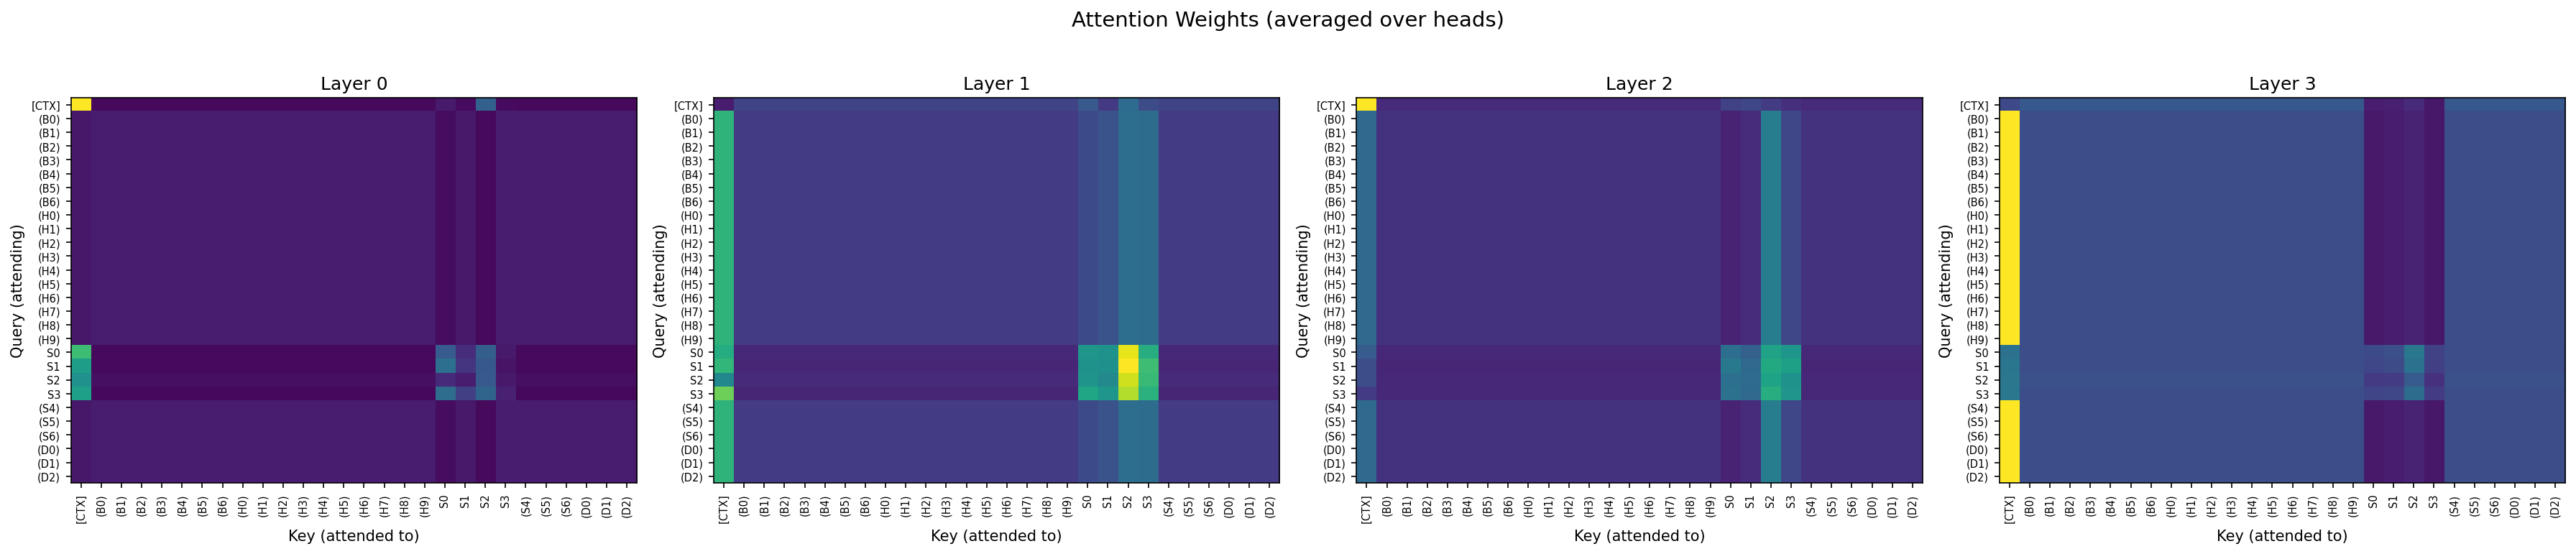
\includegraphics[width=\textwidth]{attention_avg_by_layer.png}
  \caption{Средневзвешенные карты внимания по слоям Transformer-агента. На Layer~0 внимание концентрируется на юнитах доски (B0--B6) и токене контекста [CTX]; на Layer~3 формируются устойчивые паттерны кросс-зонного взаимодействия между доской и магазином}
  \label{fig:attention_layers}
\end{figure}

\begin{figure}[H]
  \centering
  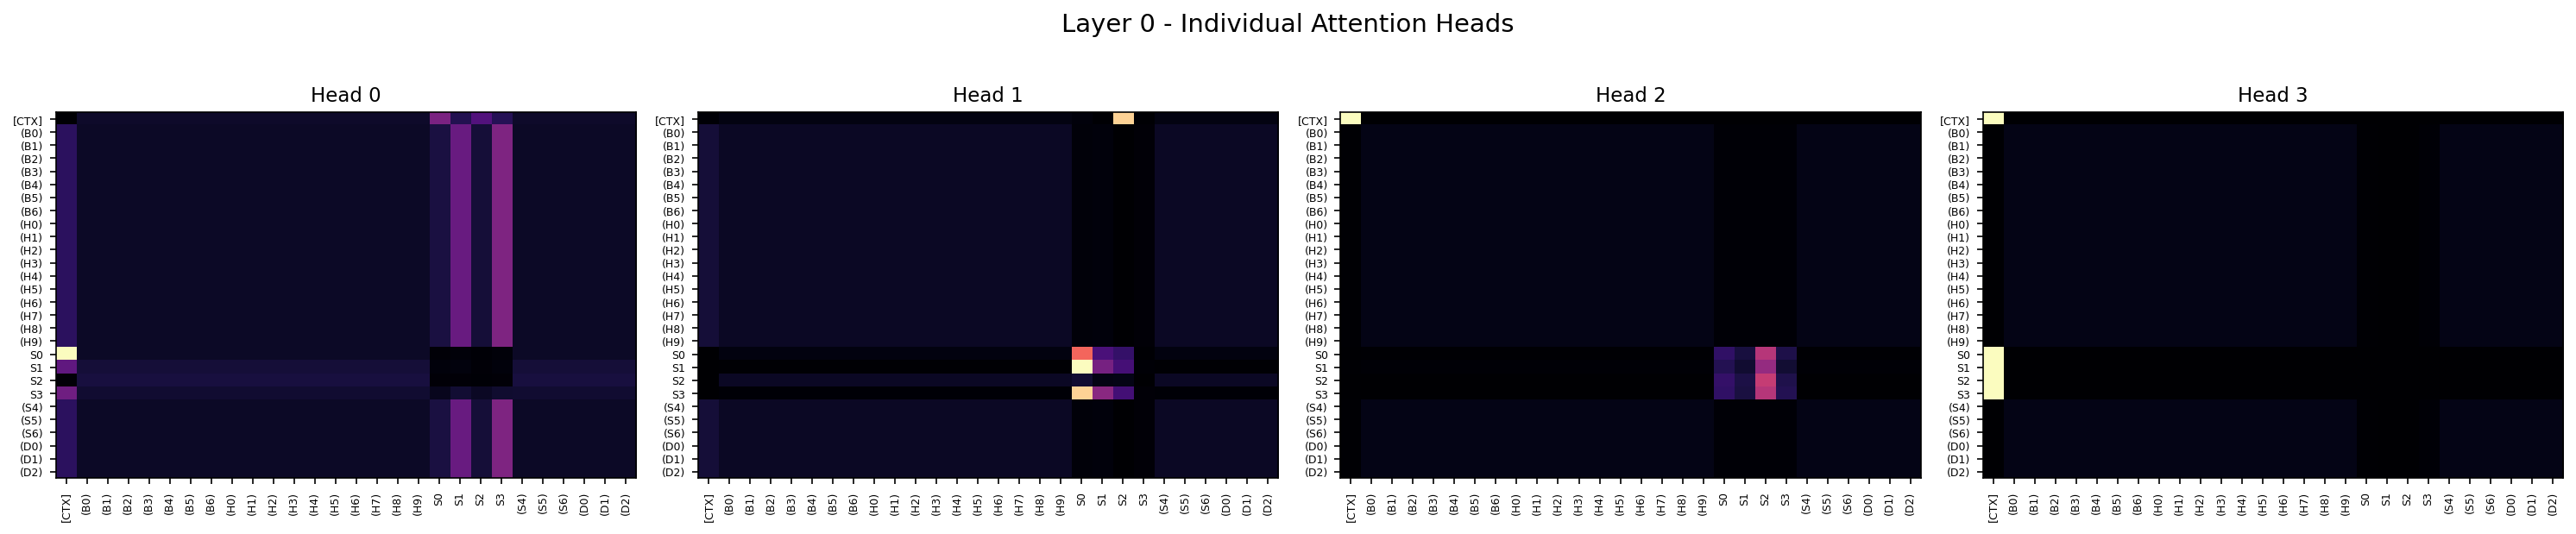
\includegraphics[width=\textwidth]{attention_heads_layer0.png}
  \caption{Карты внимания отдельных голов Layer~0. Head~0 специализируется на внутридосковых связях; Head~1 фокусируется на слотах магазина; Head~3 --- на глобальном контексте и Discovery-зоне}
  \label{fig:attention_heads}
\end{figure}

\subsection{Детерминированность}

Для научной воспроизводимости экспериментов реализована функция \texttt{setup\_determinism(seed)}, устанавливающая:
\begin{itemize}[noitemsep]
  \item \texttt{PYTHONHASHSEED} для детерминированного хеширования;
  \item \texttt{CUBLAS\_WORKSPACE\_CONFIG} для детерминированных CUDA-операций;
  \item \texttt{torch.backends.cudnn.deterministic = True};
  \item \texttt{set\_random\_seed()} из SB3 для NumPy, PyTorch и Python random.
\end{itemize}

\newpage

% ==================== 6. EXPERIMENTS ====================
\section{Эксперименты и результаты}

\subsection{Цели экспериментов}

Экспериментальная часть преследует три цели:
\begin{enumerate}[noitemsep]
  \item \textbf{Валидация среды}: подтверждение корректности формирования наблюдений, масок, наград и прохождения градиентов;
  \item \textbf{Демонстрация сходимости}: обученный агент должен демонстрировать осмысленное поведение (покупка юнитов, заполнение доски, использование триплетов);
  \item \textbf{Сравнение архитектур}: оценка преимуществ Transformer-экстрактора по сравнению с MLP-baseline.
\end{enumerate}

\subsection{Конфигурация экспериментов}

Основные параметры обучения для обеих архитектур сведены в Таблице~\ref{tab:experiment_config}.

\begin{longtable}{p{5.5cm}p{4cm}p{4cm}}
\caption{Конфигурация экспериментов}\label{tab:experiment_config}\\
\toprule
\textbf{Параметр} & \textbf{MLP Baseline} & \textbf{Transformer} \\
\midrule
Алгоритм & MaskablePPO & MaskablePPO \\
Архитектура & MLP $[512, 512]$ & Transformer (4L, 4H, 128D) \\
Learning Rate & $3 \times 10^{-4}$ & $3 \times 10^{-4}$ \\
$\gamma$ (discount) & $0.99$ & $0.99$ \\
Batch Size & 256 & 256 \\
$n\_steps$ & 2\,048 & 2\,048 \\
Entropy Coefficient & 0.01 & 0.01 \\
Параллельные среды & 4 & 4 \\
Всего шагов & 1\,500\,000 & 300\,000 \\
GPU & T4 (Kaggle) & T4 (Kaggle) \\
Self-Play & 50\,000 шагов & 50\,000 шагов \\
Zero-Init & Нет & Да (Actor + Critic) \\
\bottomrule
\end{longtable}

\subsection{Результаты обучения}

\subsubsection{Метрики сходимости}

Ключевым экспериментальным результатом является \textbf{скорость сходимости} (sample efficiency). Результаты сведены в Таблице~\ref{tab:sample_efficiency}. Обе архитектуры были обучены до достижения плато по метрике \texttt{avg\_board\_power} $\approx 15$:

\begin{longtable}{p{6cm}p{3.5cm}p{3.5cm}}
\caption{Сравнение скорости сходимости (Sample Efficiency)}\label{tab:sample_efficiency}\\
\toprule
\textbf{Метрика} & \textbf{MLP} & \textbf{Transformer} \\
\midrule
Шаги до плато ($\sim$15 board power) & $\sim$400\,000 & \textbf{$\sim$80\,000} \\
\textbf{Ускорение (sample efficiency)} & 1$\times$ & \textbf{$\sim$5$\times$} \\
Inference speed & $\sim$600 fps & $\sim$200 fps \\
\bottomrule
\end{longtable}

\textbf{Transformer сходится в $\sim$5 раз быстрее по количеству шагов обучения.} При этом каждый шаг Transformer-итерации дороже вычислительно ($\sim$3$\times$ медленнее per iteration из-за $O(N^2)$ Self-Attention), но суммарная выгода по числу необходимых взаимодействий со средой (Net Sample Efficiency) остаётся в пользу Transformer.

\subsubsection{Метрики MLP-baseline на плато (1.5M шагов)}

\begin{longtable}{p{5cm}p{3cm}p{5.5cm}}
\caption{Метрики MLP-baseline на плато (1.5M шагов)}\label{tab:mlp_metrics}\\
\toprule
\textbf{Метрика} & \textbf{Значение} & \textbf{Интерпретация} \\
\midrule
Explained Variance & $\sim$0.7 & Value function корректно предсказывает return \\
Value Loss & $\sim$3.0 & Стабильная оценка value с высокой дисперсией \\
Policy Gradient Loss & $\sim$$-0.03$ & Стабильная оптимизация политики \\
Entropy Loss & $\sim$$-0.85$ & Политика уверена в решениях \\
Avg Board Power & $\sim$15 & Потолок текущей конфигурации среды \\
\bottomrule
\end{longtable}

\texttt{explained\_variance} $\approx 0.7$ говорит о том, что Critic неплохо предсказывает return --- вся цепочка <<среда $\to$ obs $\to$ нейросеть $\to$ gradient>> работает. По поведению оба агента играют осмысленно: покупают юнитов, заполняют доску до 7 слотов, собирают триплеты и через Triple Reward берут карты высоких тиров.

\emph{Замечание}: Transformer обучался 300K шагов (лимит GPU Kaggle T4), MLP --- 1.5M. Тем не менее Transformer вышел на плато за $\sim$5$\times$ меньше сэмплов.

\subsubsection{PvP: Transformer vs MLP}

Мы стравили обученных агентов (MLP после 1.5M шагов, Transformer после 300K) через \texttt{evaluate\_pvp.py} (Таблица~\ref{tab:pvp_results}):

\begin{longtable}{p{3cm}p{3cm}p{3cm}p{3cm}}
\caption{Результаты прямого столкновения Transformer vs MLP}\label{tab:pvp_results}\\
\toprule
\textbf{Игра} & \textbf{HP Transformer} & \textbf{HP MLP} & \textbf{$\Delta$HP} \\
\midrule
1 & 22 & 21 & $+1$ \\
2 & 30 & 25 & $+5$ \\
3 & 24 & 27 & $-3$ \\
\bottomrule
\end{longtable}

Главный результат PvP: \textbf{все три матча ушли в таймаут} ($>$500 ходов). Ни один агент не смог убить другого --- HP колебалось в районе 20--30 на протяжении всей партии.

Что из этого следует:

\begin{enumerate}[noitemsep]
  \item \textbf{Обе архитектуры <<решили>> задачу}: и MLP, и Transformer научились строить максимально живучие доски. При 18 юнитах и тирах 1--3 пространство стратегий не настолько велико, чтобы разница в архитектуре дала преимущество в PvP;
  \item \textbf{Среда слишком простая}: то, что MLP и Transformer играют одинаково сильно, говорит скорее о потолке сложности нашей среды. Чтобы Transformer мог показать себя, нужно больше карт и кросс-расовые синергии;
  \item \textbf{Среда реализована корректно}: сам факт стабильного равновесия --- хороший знак. Агенты не нашли эксплойтов, не зациклились, а выработали осмысленную стратегию --- значит, движок работает правильно.
\end{enumerate}

\subsection{Анализ сходимости}

Ни MLP, ни Transformer не показали катастрофического забывания или коллапса политики --- обучение шло стабильно на всём протяжении. Мы выделили три характерные фазы (границы даны для MLP; Transformer проходит те же этапы примерно в 5 раз быстрее):

\begin{enumerate}[noitemsep]
  \item \textbf{<<Научиться тратить золото>>} (MLP: 0--200K, Transformer: 0--40K): агент понимает, что надо покупать юнитов, когда есть деньги, и жать End Turn, когда денег нет. Board Power растёт с 0 до $\sim$8;
  \item \textbf{<<Синергии и триплеты>>} (MLP: 200K--800K, Transformer: 40K--160K): появляются расовые связки, сбор триплетов, использование Discovery. Board Power доходит до $\sim$13;
  \item \textbf{<<Финальная шлифовка>>} (MLP: 800K--1.5M, Transformer: 160K--300K): агент учится тонкостям --- когда повышать тир таверны, как расставлять юнитов. Board Power выходит на плато $\sim$15--18.
\end{enumerate}

Динамика обучения наглядно представлена на Рисунке~\ref{fig:wandb_training}: кривые loss-функций демонстрируют устойчивое снижение, при этом Transformer (розовая линия) сходится существенно быстрее MLP-baseline (оранжевая линия).

\begin{figure}[H]
  \centering
  \includegraphics[width=0.95\textwidth]{wandb_page0.png}
  \caption{Динамика ключевых метрик обучения (WandB): value\_loss, policy\_gradient\_loss и train\_loss для MLP (оранжевая) и Transformer (розовая). Transformer достигает стабильных значений loss в $\sim$5 раз быстрее по числу шагов}
  \label{fig:wandb_training}
\end{figure}

\begin{figure}[H]
  \centering
  \includegraphics[width=0.95\textwidth]{wandb_page3.png}
  \caption{Динамика board\_power (WandB): максимальная и средняя сила доски агентов. Transformer (розовая) достигает плато ($\sim$15) на порядок быстрее MLP (оранжевая), подтверждая преимущество в sample efficiency}
  \label{fig:board_power}
\end{figure}

Помимо фазовой структуры, наблюдался \textbf{эффект Self-Play}: после обновления оппонента (каждые 50\,000 шагов) фиксировались кратковременные просадки value loss --- агент адаптируется к новому стилю игры противника, --- после чего метрики стабилизировались на более высоком уровне.

GTrXL-шлюзы и Zero-Init FiLM были включены в архитектуру на основе теоретических рекомендаций из~\cite{gtrxl} и~\cite{dreamerv3} соответственно. Полноценный ablation study (отключение отдельных компонентов) не проводился из-за ограничений вычислительных ресурсов и является предметом дальнейшей работы.

\newpage

% ==================== 7. TESTING ====================
\section{Тестирование}

Корректность реализации движка подтверждена обширным набором из \textbf{13 тестовых модулей} общим объёмом нескольких тысяч строк. Тесты организованы по принципу ``белого ящика'' и покрывают:

\begin{itemize}[noitemsep]
  \item \textbf{Модульные тесты сущностей} (\texttt{test\_entities.py}): создание юнитов из базы данных, многоуровневая система баффов (перманентные, ходовые, боевые, аурные), корректность Golden-версий с удвоенными статами, механика Magnetize (объединение Mech-юнитов с суммированием баффов и attached-эффектов), метод \texttt{restore\_stats()} с сохранением потери HP;
  \item \textbf{Тесты системы событий} (\texttt{test\_event\_system.py}): корректность порядка триггеров (group $\to$ priority $\to$ side $\to$ slot $\to$ uid), вложенные цепочки (Deathrattle $\to$ SUMMONED $\to$ Deflect-o-Bot trigger), обработка Golden-юнитов (двойное срабатывание), корректность EffectContext (buff\_perm, summon, gain\_gold);
  \item \textbf{Тесты боевой системы} (\texttt{test\_combat.py}): Deathrattle + Reborn (призыв копии с 1 HP после смерти), Cleave (урон по 3 юнитам одновременно), Divine Shield (поглощение первого удара), Poisonous/Venomous (мгновенное убийство), Windfury (двойная атака), Immediate Attack (внеочередная атака токена), Taunt-приоритет, корректность вычисления урона герою;
  \item \textbf{Тесты таверны} (\texttt{test\_tavern.py}): покупка (проверка золота, места в руке), продажа (возврат золота и карт в пул), триплеты (слияние 3 копий с суммированием баффов, выдача Triple Reward), Discovery (выбор из 3 уникальных карт, изъятие из пула, возврат невыбранных), заморозка магазина, апгрейд таверны, розыгрыш заклинаний (таргетированных и нетаргетированных);
  \item \textbf{Тесты пула карт} (\texttt{test\_pool.py}): конечность запаса (изъятие и возврат копий), вероятностная выборка по тирам, Discovery с unique constraint;
  \item \textbf{Интеграционные тесты} (\texttt{test\_integration.py}): полные партии от начала до определения победителя, корректность Self-Play (два агента с разными стратегиями);
  \item \textbf{Тесты RL-среды} (\texttt{test\_rl\_env.py}): корректность Action Masking (все невозможные действия замаскированы), формирование наблюдений (размерность 1009, нормализация значений), корректность reset/step циклов;
  \item \textbf{Тесты Golden-логики} (\texttt{test\_golden\_logic.py}): полный цикл триплетов для каждого юнита, корректность golden Battlecry (например, Golden Alleycat призывает Golden Tabbycat);
  \item \textbf{Тесты новых механик} (\texttt{test\_new\_mechanics.py}): Kaboom Bot (4 урона случайному врагу), Deflect-o-Bot (DS при призыве мехов), Spawn of N'Zoth (+1/+1 всем при смерти);
  \item \textbf{Тесты покрытия пробелов} (\texttt{test\_coverage\_gaps.py}): пограничные случаи --- пустая доска при продаже, переполнение руки, Discovery при пустом пуле.
\end{itemize}

\newpage

% ==================== 8. LIMITATIONS ====================
\section{Ограничения и направления дальнейшей работы}

\subsection{Текущие ограничения}

\begin{enumerate}[noitemsep]
  \item \textbf{Ограниченный пул карт}: текущая реализация покрывает подмножество юнитов и заклинаний первых тиров; в оригинальной игре представлено свыше 200 уникальных карт тиров 1--6. Расширение пула является приоритетной задачей, при этом архитектура движка \emph{не требует модификации} --- достаточно добавить записи в \texttt{CARD\_DB} и триггеры в \texttt{TRIGGER\_REGISTRY};
  \item \textbf{Формат 1v1}: симулируется дуэль двух игроков, тогда как оригинал предполагает 8 участников с ротацией пар. Расширение до 8 игроков потребует модификации класса \texttt{Game} и среды, но не затронет ядро движка;
  \item \textbf{Вычислительные ресурсы}: обучение проводилось на NVIDIA Tesla T4 (16 GB VRAM, Kaggle), что ограничило длительность экспериментов и не позволило провести полноценный ablation study;
  \item \textbf{Отсутствие героев}: в оригинальной игре каждый игрок выбирает героя с уникальной Hero Power, создающей дополнительный слой стратегического разнообразия;
  \item \textbf{Эволюция метагейма}: Hearthstone Battlegrounds регулярно обновляется разработчиком --- добавляются новые юниты, расы, механики и заклинания, что непрерывно увеличивает комбинаторную сложность среды. Поддержание актуальности симулятора потребует систематического обновления базы данных карт и реестра триггеров.
\end{enumerate}

\subsection{Направления дальнейшей работы}

Проект задумывался как исследовательская платформа, а не как конечный продукт. Ниже --- конкретные направления, в которые мы планируем двигаться.

\subsubsection{Расширение Action Space}

Сейчас действие --- один элемент из Discrete(32). При расширении пула карт это перестанет работать. Решение --- \textbf{авторегрессионная декомпозиция} по схеме SAINT~\cite{saint}: агент сначала выбирает тип действия, затем источник через Pointer Network~\cite{pointer}, затем цель. Это снижает сложность с $O(\prod |A_i|)$ до $O(\sum |A_i|)$, плюс Roll и End Turn можно завершать после первого шага, не генерируя лишних подействий.

\subsubsection{Планирование}

Стоит попробовать \textbf{Breadth-First RMCTS}~\cite{rmcts} --- GPU-батчированный MCTS, заточенный под стохастические среды. Его ключевые идеи: pre-allocated деревья в contiguous memory и prior policy для распределения бюджета. Авторы показывают $\sim$10$\times$ ускорение по сравнению с UCB-MCTS при том же бюджете.

Вторая идея --- \textbf{Latent Battle Predictor} в духе MuZero~\cite{muzero}. Вместо того чтобы симулировать бой Monte-Carlo, можно обучить сеть предсказывать исход за $O(1)$ по эмбеддингам сущностей. Оптимизация по Value Equivalence~\cite{value_equiv}: сеть не воспроизводит пошаговый бой, а сразу даёт скалярную оценку.

\subsubsection{Память и моделирование оппонента}

\textbf{Моделирование противника}~\cite{opponent}: идея --- байесовский классификатор, который по наблюдениям доски противника обновляет вероятности архетипов (<<мурлоки>>, <<мехи>> и т.д.). Агент сможет адаптировать покупки, не храня в памяти все прошлые ходы.

\textbf{DTQN}~\cite{dtqn}: Transformer Decoder, который хранит буфер из $K$ последних наблюдений. Attention напрямую достаёт нужные факты из прошлого --- без затухания, характерного для LSTM/GRU. Авторы также предлагают аугментацию $\langle\text{unk}\rangle$-токенами, чтобы сеть не <<ленилась>> и действительно использовала память.

\subsubsection{Обучающий пайплайн}

\textbf{Итеративный пайплайн BC $\to$ PPO $\to$ Self-Play}~\cite{pokemon}: вместо чистого PPO --- многоэтапная схема. Сначала коэволюционно выращиваем бота-учителя~\cite{coevolution}, затем Behavioral Cloning для прогрева весов, потом Online PPO для выхода за пределы эвристики, и наконец Self-Play для генерации нового датасета. Этапы PPO~+ Self-Play повторяются итеративно.

\textbf{Категориальный Critic (Two-Hot)}~\cite{dreamerv3}: вместо скалярного Value Head --- распределение из 255 бинов в symlog-пространстве. Это устойчивее к выбросам и позволяет работать с мультимодальными return-ами. Вдобавок Percentile Return Normalization: деление на $S = \max(\text{Perc}_{95} - \text{Perc}_{5}, 1)$ вместо стандартного $\mu/\sigma$.

\textbf{Decomposed Reward Shaping}~\cite{pokemon}: текущую функцию награды имеет смысл разложить на компоненты ($r_{\text{economy}}, r_{\text{synergy}}, r_{\text{win}}$) и постепенно убирать шейпинговые слагаемые --- иначе агент рано или поздно начнёт эксплуатировать промежуточные метрики вместо того, чтобы побеждать.

\subsubsection{Валидация подхода: Pok\'{e}mon как ближайший аналог}

Ключевым ориентиром для дальнейшего развития проекта является работа Guo et al.~\cite{pokemon}, в которой Transformer-агент достиг уровня топ-3\% рейтинговых игроков в конкурентных боях Pok\'{e}mon. Эта задача структурно близка к Hearthstone Battlegrounds:

\begin{itemize}[noitemsep]
  \item \textbf{Общие черты}: гетерогенные сущности с десятками числовых и категориальных атрибутов, стохастический исход боя (критические удары, промахи $\leftrightarrow$ рандом ударов), необходимость долгосрочного планирования (выбор команды $\leftrightarrow$ построение доски), огромное пространство карт/покемонов;
  \item \textbf{Покемоны проще}: пространство действий $|\mathcal{A}| \approx 9$ (4 атаки + switch), полная наблюдаемость своей команды, отсутствие фаз покупки/продажи и экономической подсистемы;
  \item \textbf{BG сложнее}: комбинаторное пространство действий (покупка $\times$ позиция $\times$ продажа $\times$ заклинание), неполное знание магазина (Roll как стохастический запрос), экономическое планирование (баланс gold $\leftrightarrow$ tier-up $\leftrightarrow$ freeze), фаза авто-боя без контроля.
\end{itemize}

Несмотря на существенно большую сложность BG, архитектурный пайплайн Pok\'{e}mon-агента практически полностью переносим на нашу задачу: EAV-токенизация сущностей, итеративный BC $\to$ PPO $\to$ Self-Play, Decomposed Rewards с затуханием, отказ от Decision Transformer в пользу TD-Critic из-за дисперсии боёв, и Summary Tokens для мультимодального входа. Успех данного подхода на более простой, но структурно аналогичной задаче является сильным аргументом в пользу предложенной исследовательской программы.

\newpage

% ==================== 9. CONCLUSION ====================
\section{Заключение}

Настоящая работа представляет первый этап исследовательского проекта по применению методов обучения с подкреплением к жанру автобаттлеров на примере Hearthstone Battlegrounds. Основные результаты:

\begin{enumerate}[noitemsep]
  \item \textbf{Исследовательская платформа}: спроектирован и реализован модульный headless-симулятор на Python с системой событий, боевой подсистемой с поддержкой 10 ключевых механик и экономической подсистемой (покупка, продажа, триплеты, Discovery, заклинания). Симулятор интегрирован с Gymnasium ($\mathbb{R}^{1009}$, $|\mathcal{A}| = 32$, Action Masking) и покрыт 13 тестовыми модулями;

  \item \textbf{Transformer-архитектура}: спроектирован Features Extractor, интегрирующий DecomposedEncoder, FiLM-модуляцию с Zero-Init, GTrXL-шлюзы ($z_0 \approx 0.05$), Multi-Seed PMA ($K=4$), SwiGLU FFN, RMSNorm и symlog-трансформацию;

  \item \textbf{Экспериментальная валидация}: Transformer-агент достигает эквивалентного уровня качества игры в \textbf{$\sim$5 раз быстрее} по числу шагов обучения (80K vs 400K шагов до плато). При прямом столкновении оба агента достигают устойчивого равновесия, что свидетельствует об освоении оптимальной стратегии в рамках текущей конфигурации среды.
\end{enumerate}

Полученные результаты подтверждают жизнеспособность Transformer-архитектуры для структурированных наблюдений в RL-средах с гетерогенными сущностями. Разработанная платформа спроектирована с учётом масштабируемости и не требует модификации ядра при расширении пула карт и механик. Дальнейшие направления работы --- авторегрессионная декомпозиция действий (SAINT), GPU-батчированный RMCTS, многоэтапный пайплайн BC $\to$ PPO $\to$ Self-Play и моделирование оппонента --- определяют переход от текущего PPO-baseline к агенту, способному конкурировать с опытными игроками.

\newpage

% ==================== REFERENCES ====================
\section*{Список литературы}
\addcontentsline{toc}{section}{Список литературы}

\begin{thebibliography}{99}

\bibitem{marl_gpt}
  Anonymous. MARL-GPT: Multi-Agent Reinforcement Learning with GPT~// OpenReview Submission.~---~2024.~---~Режим доступа: \url{https://anonymous.4open.science/r/marl-gpt-20365}, свободный (дата обращения: 30.03.2026).

\bibitem{opponent}
  Bursztein, E. Predicting Hearthstone Opponent Deck Using Machine Learning~// elie.net blog.~---~2018.~---~Режим доступа: \url{https://elie.net/blog/hearthstone/}, свободный (дата обращения: 30.03.2026).

\bibitem{dtqn}
  Esslinger, K., Platt, R., Amato, C. Deep Transformer Q-Networks for Partially Observable Reinforcement Learning~// arXiv preprint.~---~2022.~---~arXiv:2206.01078.~---~Режим доступа: \url{https://arxiv.org/abs/2206.01078}, свободный (дата обращения: 30.03.2026).

\bibitem{coevolution}
  Garc\'{i}a-S\'{a}nchez, P. et al. Evolutionary Optimization of Hearthstone Agents~// arXiv preprint.~---~2024.~---~arXiv:2410.19681.~---~Режим доступа: \url{https://arxiv.org/abs/2410.19681}, свободный (дата обращения: 30.03.2026).

\bibitem{pokemon}
  Guo, Y. et al. Pok\'{e}mon Agent: Reinforcement Learning for Turn-Based Strategy Games~// arXiv preprint.~---~2025.~---~arXiv:2504.04395.~---~Режим доступа: \url{https://arxiv.org/abs/2504.04395}, свободный (дата обращения: 30.03.2026).

\bibitem{dreamerv3}
  Hafner, D., Pasukonis, J., Ba, J., Lillicrap, T. Mastering Diverse Domains through World Models~// arXiv preprint.~---~2023.~---~arXiv:2301.04104.~---~Режим доступа: \url{https://arxiv.org/abs/2301.04104}, свободный (дата обращения: 30.03.2026).

\bibitem{set_transformer}
  Lee, J., Lee, Y., Kim, J. et al. Set Transformer: A Framework for Attention-based Permutation-Invariant Input~// Proceedings of ICML.~---~2019.~---~arXiv:1810.00825.~---~Режим доступа: \url{https://arxiv.org/abs/1810.00825}, свободный (дата обращения: 30.03.2026).

\bibitem{survey_trl}
  Li, W. et al. A Survey on Transformers in Reinforcement Learning~// arXiv preprint.~---~2023.~---~arXiv:2307.05979.~---~Режим доступа: \url{https://arxiv.org/abs/2307.05979}, свободный (дата обращения: 30.03.2026).

\bibitem{rmcts}
  Luo, S. et al. Breadth-First RMCTS: GPU-Batched Monte-Carlo Tree Search~// arXiv preprint.~---~2025.~---~arXiv:2601.01301.~---~Режим доступа: \url{https://arxiv.org/abs/2601.01301}, свободный (дата обращения: 30.03.2026).


\bibitem{value_equiv}
  Oh, J. et al. Discovering Object-Centric Generalized Value Functions From Pixels~// arXiv preprint.~---~2022.~---~arXiv:2209.00588.~---~Режим доступа: \url{https://arxiv.org/abs/2209.00588}, свободный (дата обращения: 30.03.2026).

\bibitem{openai_five}
  OpenAI. Dota 2 with Large Scale Deep Reinforcement Learning~// arXiv preprint.~---~2019.~---~arXiv:1912.06680.~---~Режим доступа: \url{https://arxiv.org/abs/1912.06680}, свободный (дата обращения: 30.03.2026).

\bibitem{gtrxl}
  Parisotto, E., Song, H.~F., Rae, J.~W. et al. Stabilizing Transformers for Reinforcement Learning~// Proceedings of ICML.~---~2020.~---~arXiv:1910.06764.~---~Режим доступа: \url{https://arxiv.org/abs/1910.06764}, свободный (дата обращения: 30.03.2026).

\bibitem{film}
  Perez, E., Strub, F., de Vries, H. et al. FiLM: Visual Reasoning with a General Conditioning Layer~// Proceedings of AAAI.~---~2018.~---~Режим доступа: \url{https://arxiv.org/abs/1709.07871}, свободный (дата обращения: 30.03.2026).

\bibitem{hs_leiden}
  Ren, S. Reinforcement Learning for Hearthstone Battlegrounds~// Leiden University, LIACS.~---~2022.~---~Режим доступа: \url{https://theses.liacs.nl/2366}, свободный (дата обращения: 30.03.2026).

\bibitem{scale_anchoring}
  Rybkin, O. et al. Scale Anchoring for Stable PPO Training with Transformers~// arXiv preprint.~---~2026.~---~arXiv:2602.10408.~---~Режим доступа: \url{https://arxiv.org/abs/2602.10408}, свободный (дата обращения: 30.03.2026).

\bibitem{muzero}
  Schrittwieser, J., Antonoglou, I., Hubert, T. et al. Mastering Atari, Go, Chess and Shogi by Planning with a Learned Model~// Nature.~---~2020.~---~Vol.~588.~---~P.~604--609.~---~Режим доступа: \url{https://arxiv.org/abs/1911.08265}, свободный (дата обращения: 30.03.2026).

\bibitem{swiglu}
  Shazeer, N. GLU Variants Improve Transformer~// arXiv preprint.~---~2020.~---~arXiv:2002.05202.~---~Режим доступа: \url{https://arxiv.org/abs/2002.05202}, свободный (дата обращения: 30.03.2026).

\bibitem{vieira2022}
  Vieira, R., Tavares, A.~R., Chaimowicz, L. Exploring Deep Reinforcement Learning for Battling in Collectible Card Games~// Proceedings of SBGames.~---~2022.~---~Режим доступа: \url{https://doi.org/10.1109/SBGAMES56371.2022.9961110}, свободный (дата обращения: 30.03.2026).

\bibitem{alphastar}
  Vinyals, O., Babuschkin, I., Czarnecki, W.~M. et al. Grandmaster level in StarCraft II using multi-agent reinforcement learning~// Nature.~---~2019.~---~Vol.~575.~---~P.~350--354.~---~Режим доступа: \url{https://www.nature.com/articles/s41586-019-1724-z}, свободный (дата обращения: 30.03.2026).

\bibitem{pointer}
  Vinyals, O., Fortunato, M., Jaitly, N. Pointer Networks~// Proceedings of NeurIPS.~---~2015.~---~arXiv:1506.03134.~---~Режим доступа: \url{https://arxiv.org/abs/1506.03134}, свободный (дата обращения: 30.03.2026).

\bibitem{saint}
  Wen, C. et al. SAINT: Scalable Autoregressive Interaction Network for Transformer Agents~// arXiv preprint.~---~2025.~---~arXiv:2505.12109.~---~Режим доступа: \url{https://arxiv.org/abs/2505.12109}, свободный (дата обращения: 30.03.2026).

\bibitem{preln}
  Xiong, R., Yang, Y., He, D. et al. On Layer Normalization in the Transformer Architecture~// Proceedings of ICML.~---~2020.~---~arXiv:2002.04745.~---~Режим доступа: \url{https://arxiv.org/abs/2002.04745}, свободный (дата обращения: 30.03.2026).

\bibitem{rmsnorm}
  Zhang, B., Sennrich, R. Root Mean Square Layer Normalization~// Proceedings of NeurIPS.~---~2019.~---~arXiv:1910.07467.~---~Режим доступа: \url{https://arxiv.org/abs/1910.07467}, свободный (дата обращения: 30.03.2026).

\bibitem{hs_lut}
  Zhang, W. Design and Implementation of an Intelligent Agent for Auto Battler Games Using Reinforcement Learning~// Bachelor's Thesis, Lappeenranta--Lahti University of Technology.~---~2024.~---~Режим доступа: \url{https://lutpub.lut.fi/handle/10024/167789}, свободный (дата обращения: 30.03.2026).

\bibitem{odt}
  Zheng, Q. et al. Online Decision Transformer~// arXiv preprint.~---~2022.~---~arXiv:2202.05607.~---~Режим доступа: \url{https://arxiv.org/abs/2202.05607}, свободный (дата обращения: 30.03.2026).

\end{thebibliography}

\end{document}
